\chapter{Background}

\section{Man Group and AI in Systematic Finance}
\subsection{The Firm and its AI Deployment}
Man Group plc is a global, technology-empowered active investment management firm and the world's largest publicly listed hedge-fund firm, headquartered at Riverbank House in London. Its commercial history reaches back to 1783, when James Man founded a sugar brokerage that grew into the ED\&F Man commodities business. The modern investment business listed on the London Stock Exchange in 1994, separated from the commodities operation in 2000, and today trades under the ticker EMG as a constituent of the FTSE 250 \cite{mangroup2026about}. The firm's investment capability is organised into specialist engines that share a single technology platform: Man AHL, the quantitative and systematic arm established in 1987, with more than thirty-five years of systematic-investing heritage; Man Numeric, focused on quantitative equity; Man GLG, the discretionary business; and a solutions business providing hedge-fund and multi-manager offerings. This engine structure matters for the present work because a shared technology platform implies shared tooling.
\\\\
\textbf{AI at Man Group.} In early 2026, Man Group announced a partnership with Anthropic to deploy Claude across the business, with a stated primary focus on alpha generation and with Anthropic engineers working alongside the firm's own teams \cite{mangroup2026anthropic}. Internally, this deployment is delivered through Maia, the firm's AI platform, which provides staff with a chatbot, skills, MCP integrations, and a choice of underlying models. This estate is built and operated by the firm's AI team: a group of approximately fifteen people split across London, Boston, and Sofia, responsible for Maia, Maia Knowledge, the model and MCP integrations, and the wider rollout of AI across the business. The component of the platform most relevant to this project is Maia Knowledge, the web application through which skills are published. One architectural fact about it matters throughout this report: skills are not stored in the application's database but live in Forgejo git repositories, the firm's internal git hosting service, from which the Maia Knowledge reads and writes them over a REST API. The application's full architecture is described in Chapter 3.
\\\\
\textbf{The industrial landscape.} Man Group's adoption of AI agents sits within a broader pattern: hedge funds, and systematic managers in particular, have historically been early adopters of computational methods, and finance already possesses a mature discipline for deciding whether an opaque model can be trusted in production. That discipline is model risk management, articulated canonically in the Federal Reserve's SR 26-2 guidance \cite{federalreserve2026sr262} and extended to AI systems by the Bank of England and the Financial Conduct Authority \cite{bankofengland2022dp522}. Seen through this lens, the system described in this report is model validation applied to a new class of model artefact: a natural-language skill whose behaviour, like that of any quantitative model, must be evidenced before it is relied upon. Prior to this project, no mechanism within Man Group existed to produce that evidence.
\\\\
\subsection{AI Integrations within the firm}
Packaging internal capability as skills written in natural language is one of several ways an organisation can inject its own knowledge and workflows into a large language model system, and the choice among them is a design decision rather than a default. Four approaches dominate current practice, and they are complementary rather than mutually exclusive:

\begin{enumerate}
    \item \textbf{Fine-tuning} Adapts the weights of the model itself, either fully or through parameter-efficient methods such as low-rank adaptation (LoRA) \cite{hu2022lora}.
    \item \textbf{Retrieval-augmented generation} This approach leaves the model unchanged and supplies organisational knowledge at inference time by retrieving relevant documents into the context window \cite{lewis2020rag}.
    \item \textbf{Model Context Protocol} Connects the model to live systems through typed interfaces, so that capability resides in the tools rather than in the model or its prompt \cite{anthropic2024mcp}.
    \item \textbf{Skills} Encodes capabilities as version-controlled prose instructions that an agent loads on demand.
\end{enumerate}

All four approaches are in use at Man Group. Table \ref{tab:organisational-capability} compares the four approaches along the dimensions that matter for enterprise deployment.
\begin{table}[htbp]
    \centering
    \caption{Approaches to injecting organisational capability
    into an LLM system.}
    \label{tab:organisational-capability}

    \small
    \renewcommand{\arraystretch}{1.2}
    \setlength{\tabcolsep}{4pt}

    \begin{tabularx}{\linewidth}{
        *{5}{>{\raggedright\arraybackslash}X}
    }
        \toprule
        \textbf{Dimension}
        & \textbf{Fine-tuning}
        & \textbf{Retrieval (RAG)}
        & \textbf{Tools / MCP}
        & \textbf{Skills} \\
        \midrule

        Update process
        & Retraining
        & Update documents, index, or retrieval config
        & Modify and deploy tool code
        & Edit and distribute instructions \\

        Auditability
        & Low: behaviour encoded in weights
        & Medium: corpus inspectable, retrieval stochastic
        & High: typed interfaces, logged calls
        & High: instructions are readable prose \\
        \addlinespace

        Governance review
        & Requires behavioural testing
        & Corpus review plus behavioural testing
        & Standard code review
        & Direct human reading of instructions \\
        \addlinespace

        Cost of adding a capability
        & High (training compute and data)
        & Medium (curate and index documents)
        & Medium to high (engineering work)
        & Low (write a text file) \\

        \bottomrule
    \end{tabularx}
\end{table}

\noindent The comparison exposes the tension that motivates this project. Skills score well on precisely the dimensions a governed financial institution values: cheap to author, quickly updateable, reviewable by any literate colleague, and version-controlled with ordinary git tooling. The difficulty is that the same property producing those advantages, that a skill is prose rather than code, prevents the conventional testing instruments from transferring directly. A fine-tuned model can be benchmarked, a retrieval pipeline has measurable precision and recall, and a tool has a function signature against which unit tests can assert. Skills are not untestable in principle, but testing them requires machinery built on different foundations, which is the gap this project addresses. 

\section{Skill Harnesses and the Skill Lifecycle}
A skill needs a harness: an agent that discovers it, decides when to activate it, and follows its instructions. Within Man Group, four harnesses are available for use. Claude Code is Anthropic's command-line agent for software development and general-purpose task execution, running an interactive loop in which the model reads files, searches codebases, executes shell commands, writes and edits files, and calls further tools until a multi-step task is complete \cite{anthropic2026claudecode}, it is the harness most developers at the firm work in. The Maia chat interface gives the rest of the firm the same capabilities through a browser, so a colleague who never opens a terminal can still trigger a skill from a conversation. Additionally, two external coding agents, OpenAI's Codex and the open-source OpenCode, are also approved for use inside the firm's network. All four consume the same SKILL.md format, so a skill authored once serves every harness it is installed into, and the firm's tooling can install a skill into any of them. This breadth cuts both ways: it is what makes skills economical to author, and it is what makes a defective one costly, since a miscalibrated description or a wrong instruction propagates to every surface the skill reaches.
\\\\
Within Man Group, a skill moves through the lifecycle illustrated in Figure \ref{fig:man-group-skill-lifecycle}. An author creates a skill either locally, editing the files in their own working copy, or directly in Maia Knowledge through the browser. When the author chooses to publish, Maia Knowledge opens a pull request against the Forgejo git repository in which skills are stored. Another person reviews that pull request and merges it only if the skill is judged good, which places skills under the same review-and-merge governance the firm applies to source code. Once merged, the skill is distributed firm-wide, and any colleague can install and use it in their own harness. The lifecycle does not end there, users around the firm can continually edit skills after they are shared, and every edit re-enters the same cycle of publication, review, and distribution.
\begin{figure}
    \centering
    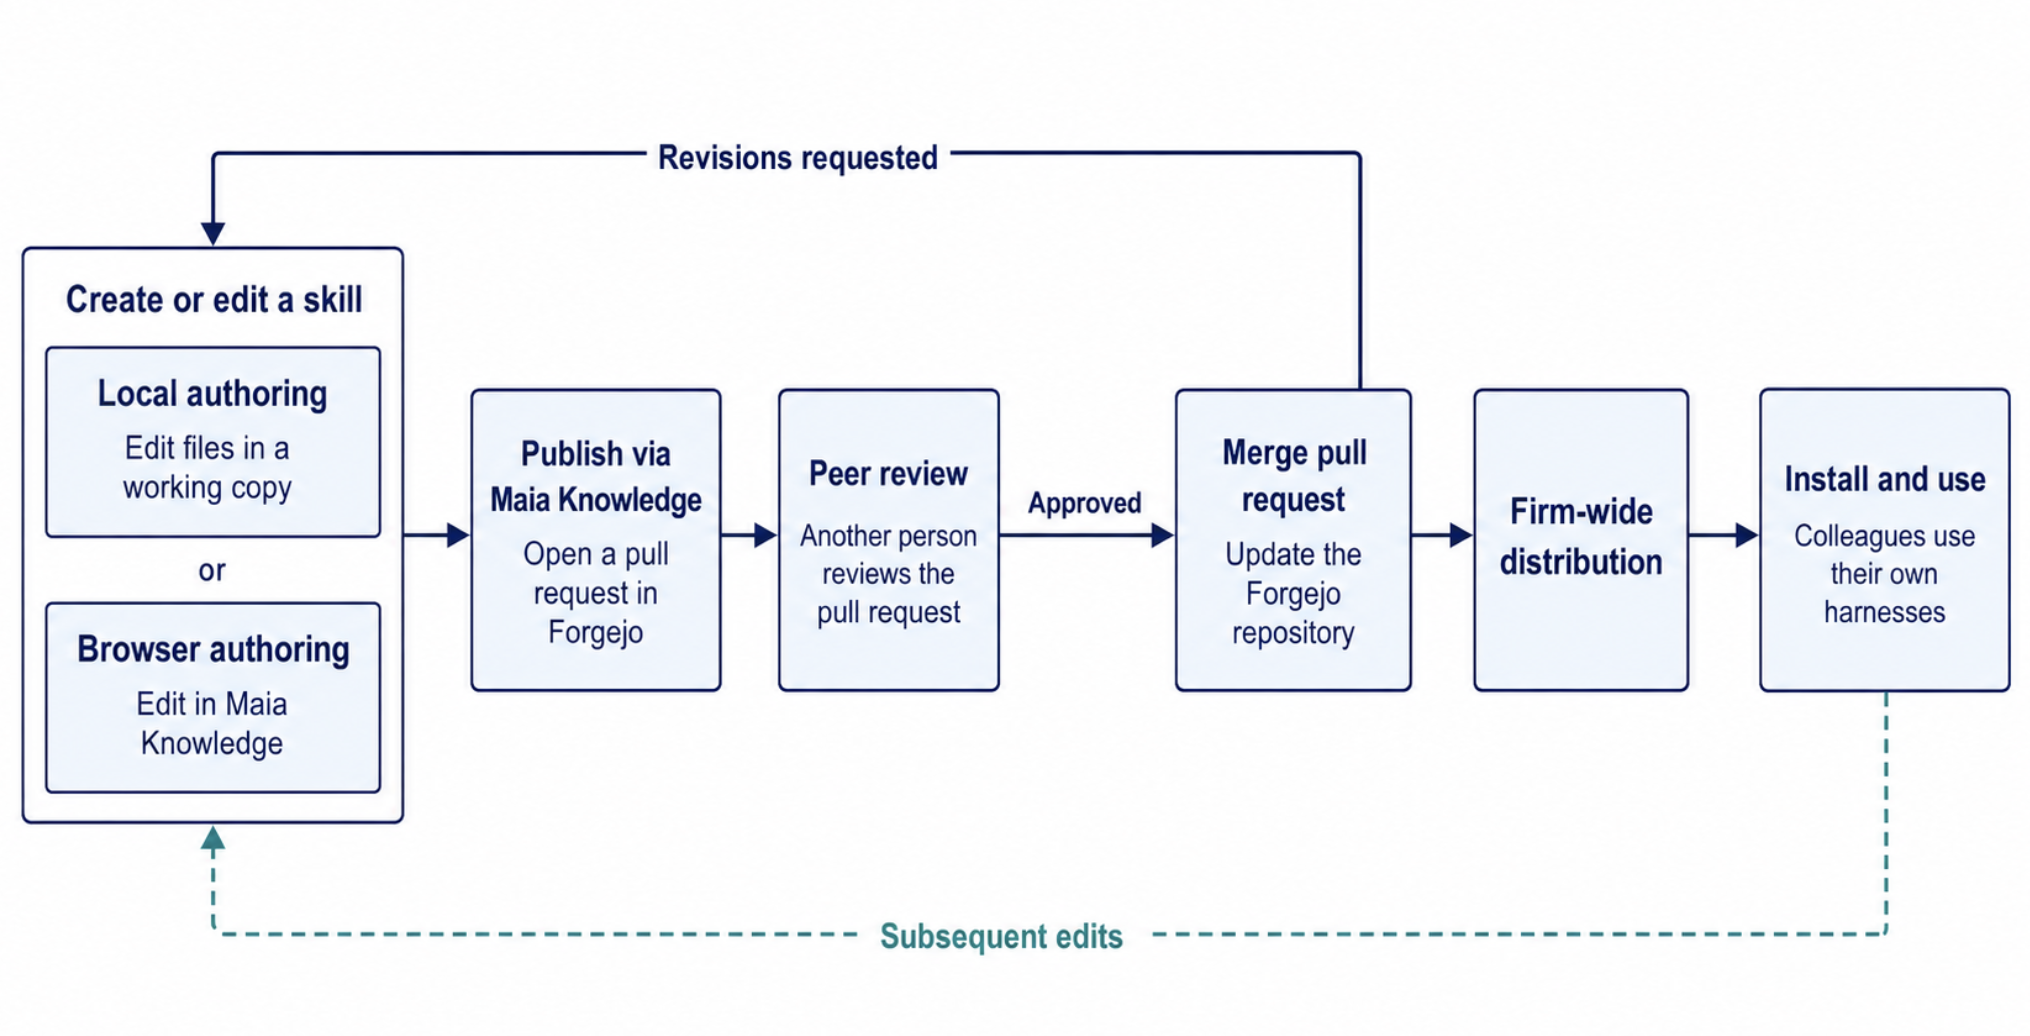
\includegraphics[width=1\linewidth]{figures/man-group-skill-lifecycle.png}
    \caption{Skill Lifecycle in Man Group}
    \label{fig:man-group-skill-lifecycle}
\end{figure}

\noindent Two things are notable about this lifecycle as it stood before this project. Nothing in it produces evidence of correct behaviour: the pull-request reviewer reads the skill's prose and judges it by eye, with no test results to consult, and the author's only way to check a skill is to try prompts against it by hand. And because editing is continuous, any confidence gained that way expires with the next change, since a reworded sentence in a published skill can silently alter behaviour for every user who has installed it. The evaluation system this report presents addresses both, inserting a testing stage between authoring and publication, highlighted in the figure.

\section{Evaluating Language-Model Outputs}

Grading a skill's output is an instance of the general problem of evaluating generated natural language. Two families of methods exist: traditional metrics that compare output against references, and language models used as judges. This section reviews both and explains why only the second fits this project's setting.

\subsection{Human Evaluation}
Human judgement is the standard against which every automatic method is measured. A competent reviewer reads the output and decides whether it is correct, complete, and useful. It is also, informally, what skill evaluation consisted of before this project, an author trying prompts by hand and reading what came back. As a method for a continuous lifecycle it fails on two counts. 

\begin{enumerate}
    \item \textbf{It does not scale:} Section 2.2 established that every edit to a published skill re-enters the cycle, and no reviewer can re-read every output of every test on every edit.
    \item \textbf{It is not consistent:} human graders disagree with one another and with themselves, and have been observed to revise what they mean by "good" as they read more outputs, a phenomenon termed criteria drift \cite{shankar2024validators}.
\end{enumerate}
 
 \noindent Human evaluation therefore keeps its role as the reference point for whether an automatic method can be trusted, and appears in that role below, but it cannot itself be the method.



\subsection{Traditional Reference-Based Metrics}
The oldest instruments for grading generated text compare a candidate against one or more human-written references. BLEU scores n-gram overlap with reference translations \cite{papineni2002bleu}, and ROUGE applies the same idea to summarisation \cite{lin2004rouge}. Both reward surface similarity rather than meaning, a limitation that later embedding-based metrics addressed. BERT Score matches candidate and reference tokens in contextual embedding space \cite{zhang2020bertscore}, while BLEURT and COMET go further and train regression models on human quality ratings \cite{sellam2020bleurt}\cite{rei2020comet}. Even before large language models, Novikova et al. showed that such automatic metrics correlate only weakly with human judgement on open-ended generation, and correlate differently across tasks and datasets \cite{novikova2017why}. 
\\\\
Two properties make this entire family unsuitable as the primary methodology for the present setting. First, all of these metrics presuppose a reference answer, and for most skill tasks no canonical reference exists. For example, the correct output of "summarise the access log in this directory" depends on the state of the environment at runtime. Second, the learned metrics are trained per task family, whereas a skill evaluation system must grade an open-ended and growing population of author-defined tasks. What the setting requires is an evaluator that can be instructed at runtime, in natural language, what to check. That is precisely the capability an LLM-as-judge provides.

\subsection{LLM-as-Judge Evaluation}

The observation that a capable language model can itself serve as the grader has produced a family of methods, and it is the family this project draws on. The premise is established: LLM evaluation of open-ended text has been shown to reproduce expert human ratings closely enough to serve as a practical substitute in settings where human evaluation is too slow or costly \cite{chiang2023llmalternative}. 
\\\\
The method most directly adopted here is G-Eval \cite{liu2023geval}. G-Eval structures judgement in two stages. In the first, an automatic chain-of-thought step: the judge model receives the task description and evaluation criteria and generates a list of concrete evaluation steps, relieving the human of writing detailed grading procedures. In the second, the judge reads the candidate output alongside those steps and emits a score in a bounded range (1-5, 1-10, etc.). The paper adds a refinement: because sampled integer scores cluster on a few values, the final score is computed as a probability-weighted sum over the score tokens, using the model's output token probabilities to obtain a finer-grained continuous value. This pipeline, with GPT-4 as the evaluator, is reported to correlate with human judgement better than every reference-based baseline across summarisation and dialogue tasks \cite{liu2023geval}. The two-stage structure, criteria first, scoring second, is the method family the judge in this project belongs to.
\\\\
Subsequent work has broadened the design space that Table \ref{tab:llm-evaluation-comparison} summarises. MT-Bench and Chatbot Arena used GPT-4 as a judge over pairwise model comparisons at scale, with reported agreement with human preferences above eighty percent while documenting the systematic biases discussed below \cite{zheng2023mtbench}. AlpacaEval automated instruction-following evaluation by having a judge compare each candidate against a fixed reference model's output, and its length-controlled revision corrects statistically for the judge's preference for longer answers \cite{li2023alpacaeval}\cite{dubois2024lengthcontrolled}. 
\\\\

\todo{Evaluate prometheus section again}
Prometheus and Prometheus 2 scores an LLM's output against a fine-grained rubric supplied by the user at evaluation time \cite{kim2024prometheus}\cite{kim2024prometheus2}. That is also the shape of the skill-evaluation problem, where what counts as a good output is defined per test by the skill's author rather than by any fixed standard, and it makes Prometheus the nearest neighbour among these systems to the judge this project needs. Its route to that capability does not transfer, however. Prometheus trains a dedicated open-weight judge model on synthetic feedback data, and it performs best when a reference answer accompanies the rubric at inference time. In this setting no bespoke judge can be trained, because the models on offer are fixed by the firm's platform, and reference answers do not exist for state-dependent skill tasks. Finally, a panel of smaller judge models has been shown to correlate with human judgement better than a single large judge while diluting any one model's biases \cite{verga2024juries}.

\begin{table}[htbp]
    \centering
    \caption{Comparison of LLM-based evaluation approaches.}
    \label{tab:llm-evaluation-comparison}
    \footnotesize
    \setlength{\tabcolsep}{3pt}
    \renewcommand{\arraystretch}{1.2}

    \begin{tabularx}{\textwidth}{
        @{}*{6}{>{\raggedright\arraybackslash}X}@{}
    }
        \toprule
        \textbf{System} &
        \textbf{Protocol} &
        \textbf{Reference required} &
        \textbf{Rubric source} &
        \textbf{Judge} \\
        \midrule

        G-Eval \cite{liu2023geval} &
        Pointwise 1 to 10 &
        No &
        Per-task criteria, auto-expanded to steps &
        Single (GPT-4) \\
        \addlinespace

        MT-Bench \cite{zheng2023mtbench} &
        Pairwise and pointwise &
        No &
        Fixed question set &
        Single (GPT-4) \\
        \addlinespace

        AlpacaEval (LC)
        \cite{li2023alpacaeval,dubois2024lengthcontrolled} &
        Pairwise vs reference model &
        Baseline outputs &
        Fixed instruction set &
        Single \\
        \addlinespace

        Prometheus 2 \cite{kim2024prometheus2} &
        Pointwise and pairwise &
        Reference answer preferred &
        User-supplied score rubric &
        Fine-tuned open judge \\
        \addlinespace

        Panel of juries \cite{verga2024juries} &
        Pointwise, aggregated &
        No &
        Task-defined &
        Multiple smaller models \\
        \addlinespace

        \bottomrule
    \end{tabularx}
\end{table}

\noindent Choosing an LLM judge means inheriting its documented failure modes, and any system that relies on judge scores has to be designed around them. Three biases recur across this literature:
\begin{enumerate}
    \item \textbf{Position bias:} The tendency to favour whichever response is presented first, is severe enough that Wang et al. could reverse many pairwise verdicts simply by swapping response order \cite{wang2024notfair}\cite{zheng2023mtbench}. 
    \item \textbf{Verbosity bias:} Favours longer answers independent of quality \cite{zheng2023mtbench}, and the length-controlled AlpacaEval revision exists precisely because this effect distorted a prominent leaderboard \cite{dubois2024lengthcontrolled}.
    \item \textbf{Self-preference bias:} LLM evaluators tend to recognise their own generations and rate them more favourably \cite{panickssery2024selfpreference}. 
\end{enumerate}

\todo{Come back to this maybe we cna just remove it}
Not all of these apply equally to skill evaluation. Position bias only occurs when two responses are compared, and a skill task produces a single output with nothing to compare it against, so the evaluation is pointwise and this bias does not arise. Verbosity bias does apply. A skill whose instructions produce longer and more elaborate answers could receive higher scores without being any more correct. Self-preference bias is the most serious of the three in this project, because the judge and the agent being judged are both Claude models, and that cannot be avoided when the whole deployment runs on one vendor. Its effect is different from the model-comparison setting in which it was first measured. There is no competitor to rank unfairly. The danger is instead a general leniency that pushes every score upward and makes any pass threshold weaker than it appears.

\todo{review from here and onwards to end of chapter 2}
\section{Testing and Evaluation of AI Agents}

Evaluating an agent differs from evaluating a text generator in three ways that shape this project. First, the unit of assessment widens from a single output to a trajectory: a sequence of tool calls, intermediate observations, and side effects, of which the final message is only the visible end. Agent-as-a-Judge makes this explicit: the evaluating system is itself an agent that inspects the evaluated agent's full working process and artefacts rather than its final answer alone, with substantial reported cost and reliability gains over judging outcomes in isolation \cite{zhuge2024agentasajudge}. Second, execution has side effects, so the evaluation harness must decide what the agent is permitted to touch, a question that returns as the containment model of Chapter 4. Third, agents are non-deterministic across repetitions of the identical task. The pass\^k metric of tau-bench quantifies this as the probability that an agent succeeds on all of k independent trials of the same task, and shows that agents which look competent at k equal to one degrade sharply as k grows \cite{yao2024taubench}. A single passing run is therefore weak evidence of a working capability, a finding whose design consequences surface in Chapters 3 and 4 and whose software-testing interpretation is taken up in Section 2.6.

\section{Agent Benchmarks}
The dominant instrument of agent evaluation is the benchmark: a fixed task suite, an environment, and a success criterion, used to compare models against one another. Table 2.3 summarises the six most influential.

\begin{table}[htbp]
    \centering
    \caption{Comparison of agent benchmarks.}
    \label{tab:agent-benchmarks}

    \small
    \renewcommand{\arraystretch}{1.2}
    \setlength{\tabcolsep}{3pt}

    \begin{tabularx}{\linewidth}{
        *{4}{>{\raggedright\arraybackslash}X}
        l
        >{\raggedright\arraybackslash}X
    }
        \toprule
        \textbf{Benchmark}
        & \textbf{Domain}
        & \textbf{Environment}
        & \textbf{Success criterion}
        & \textbf{Task set}
        & \textbf{Intended use} \\
        \midrule

        SWE-bench \cite{jimenez2024swebench}
        & Software repair
        & Real GitHub repositories
        & Held-out unit tests pass
        & Static
        & Compare models on issue resolution \\
        \addlinespace

        WebArena \cite{zhou2024webarena}
        & Web tasks
        & Self-hosted realistic websites
        & Programmatic state checks
        & Static
        & Compare web agents \\
        \addlinespace

        GAIA \cite{mialon2024gaia}
        & General assistance
        & Tools, web, files
        & Exact match to factoid answer
        & Static
        & Compare general assistants \\
        \addlinespace

        ToolLLM \cite{qin2024toolllm}
        & API use
        & 16,000+ real REST APIs
        & Judge-assessed solvability
        & Static
        & Compare tool-use ability \\
        \addlinespace

        AgentBench \cite{liu2024agentbench}
        & Multi-domain
        & Eight simulated environments
        & Per-environment metrics
        & Static
        & Compare LLMs as agents \\
        \addlinespace

        OSWorld \cite{xie2024osworld}
        & Computer use
        & Real operating systems
        & Execution-based state checks
        &
        & \\

        \bottomrule
    \end{tabularx}
\end{table}

Two features of this landscape matter here. The first is the ingenuity of the success criteria: SWE-bench grades with held-out unit tests, WebArena and OSWorld with programmatic checks on environment state, GAIA with exact match against questions deliberately constructed to have single factual answers. Each of these is a way of manufacturing a deterministic oracle, and each purchases it by constraining the task distribution to tasks that admit one. An open-ended skill task graded by an author's rubric admits no such construction, which is why this project inherits the judge of Section 2.3 rather than the oracles of Table 2.3. The second feature is the critique the benchmarks have attracted. A prominent critique argues that agent benchmarking as practised is cost-blind, reporting accuracy without the token expenditure needed to reach it, encourages overfitting to leaderboards, and often lacks adequate holdout sets, so that reported gains do not transfer \cite{kapoor2025agentsmatter}. Its prescription, that evaluation should be designed for its downstream decision rather than for ranking, describes this project's purpose exactly: the decision is not which model is best but whether this version of this skill is fit to publish.

Placing this project against the surveyed work is clarified by two axes: what is compared, and when. On the first axis, every benchmark in Table 2.3 compares models against each other on a fixed task suite, whereas this system compares versions of a single capability against its own test suite, holding the model constant. On the second axis, a benchmark is run episodically, when a new model appears, whereas the evaluations here run continuously through a skill's authoring lifecycle, on every edit that might regress behaviour. The combination, continuous regression evaluation of a versioned natural-language capability, is occupied by none of the surveyed work. One further absence is sharper still. In every benchmark above, the task is handed to the agent directly, so the question of whether the agent would have chosen to engage the right capability never arises. Yet Section 1.2 established that wrong activation is one of the two failure modes that actually occur in deployment, and Section 2.2 showed that activation depends on a single description field. To the best of the author's knowledge, no published evaluation framework tests activation against the live capability-selection mechanism, and the invocation dimension of this project has no direct academic precedent. Whether practitioner tooling fills either gap is the question of the next section.

\section{Evaluation Tooling in Practice}
\subsection{The Tooling Landscape}
Outside the academic literature, a substantial ecosystem of evaluation tooling has grown around production LLM systems, and the honest question for an industrial project is why any of it was not simply adopted. OpenAI Evals established the practitioner template of a registry of test cases with pluggable graders, including model-based ones \cite{openai2023evals}. Inspect, from the UK AI Security Institute, is the closest in spirit to the present work: a rigorously engineered Python framework in which an evaluation is a composition of a dataset, a solver, and a scorer, with first-class support for agentic tool use and model-graded scoring \cite{aisi2024inspect}. DeepEval packages LLM-as-judge metrics, G-Eval among them, behind a pytest-style interface \cite{confidentai2024deepeval}, and promptfoo targets rapid comparison of prompts and models from configuration files \cite{promptfoo2024}. LangSmith embeds evaluation into an observability platform, tracing production calls and scoring them against datasets \cite{langchain2024langsmith}. Alongside these general frameworks sits a genre of domain-specific evaluators, exemplified by Ragas, which grades retrieval-augmented generation pipelines on retrieval-specific dimensions such as faithfulness and context relevance \cite{es2024ragas}; its existence illustrates that evaluation machinery tends to specialise around the architecture it serves, which is equally true of the system described here.


\subsection{Requirements of This Setting}
The decision to build rather than adopt was a requirements decision, not a judgement that these tools are deficient at what they do. Five requirements had to hold jointly. (i) Activation must be tested against the live skill-discovery mechanism, which requires running the real Claude Code agent with the skill installed and observing whether the Skill tool fires; a framework that evaluates through a chat-completion API never exercises the mechanism whose miscalibration is the failure mode under test. (ii) The skill under test must be materialised from its Forgejo repository inside the firm's authenticated perimeter, since skills are git artefacts (Section 2.1) and evaluation must grade exactly the version under review. (iii) One evaluation engine must serve the Skill Manager web interface, the command-line tool, and future continuous-integration use identically, so that a passing score means the same thing wherever it was produced; a tool that lives only in a notebook or only in a hosted dashboard cannot give that guarantee. (iv) The agent under test must be isolated from its own answer key, because the test configuration containing every prompt and rubric sits in the same repository as the skill, a hazard that shared-corpus evaluation frameworks do not face and therefore do not defend against. (v) Results must flow into the governance workflow of Section 2.2, attached to the skill version a reviewer is approving. Each surveyed tool satisfies some of these requirements; none satisfies all five, and the first, activation testing, is satisfied by none individually, consistent with the academic gap identified in Section 2.4.
\\\\
The conclusion this survey supports is deliberately modest. The judge methodology of this project is adopted from the literature, and its workflow concepts, test registries, model-graded scoring, configuration-as-code, are shared with the practitioner tools above. The contribution is the integration of both under the five joint constraints, which none of the existing systems was built to meet. The workflow being integrated into, testing on change and gating release, comes from software engineering, whose perspective the next section examines.

\section{Legal, Social, Ethical and Professional Considerations}
\subsection{Legal and Regulatory Context}
The regulatory framing introduced in Section 2.1 does the legal work here: within a systematic investment firm, an evaluation score is not a curiosity but an input to a governed decision about whether an AI capability may be relied upon, and the surrounding supervisory expectations on model risk make the firm accountable for that decision \cite{federalreserve2026sr262}\cite{bankofengland2022dp522}. This assigns the evaluation system a specific ethical burden: the evidence it produces must be honest about its own reliability, because a governance reviewer will treat it as evidence. At the European level, the EU AI Act establishes a risk-tiered regime whose heaviest obligations attach to enumerated high-risk uses \cite{eu2024aiact}; an internal skill-testing tool does not sit in those categories, but the Act's underlying expectations of documentation, transparency, and human oversight describe the standard this project holds itself to voluntarily.

\subsection{Professional and Ethical Practice}
The most concrete ethical hazard in this project is over-trust: a numeric score with a pass verdict invites more confidence than an approximate oracle warrants. Several deliberate practices respond to that hazard, and they are professional-practice decisions as much as engineering ones. Tool-enabled evaluation prints an unsuppressable disclosure banner stating its tool surface and the limits of its containment before any run, because a mode with real side effects must never run without the operator's knowledge. Out-of-range judge scores are retried and then errored, never clamped into validity, because a silently repaired score misrepresents what the judge said. Most consequentially, when governance review exposed that a nonsense rubric could score ninety percent, the finding was documented, root-caused, and published internally alongside a redesign proposal rather than minimised; Chapters 5 and 6 present it in the same spirit. Reporting the limitations of one's own system with the same rigour as its capabilities is the conduct that professional codes in computing require, and this report treats it as a requirement rather than an aspiration.

\subsection{Data and Social Considerations}
Evaluation traffic carries the firm's information: test prompts and rubrics routinely embed internal terminology, procedures, and system names. All model calls therefore travel through the firm's approved internal gateway rather than public endpoints, results are stored in an access-controlled internal database, and tool-enabled runs reach internal systems only under the classifier-reviewed permission mode described in Chapter 4. The social dimension is internal but real: skills installed from the marketplace shape how colleagues across the firm work, and a defective skill silently propagates its defects to every installer. An evaluation gate at publication is thus a protection for the many users who inherit a skill, not merely a convenience for its author. These considerations recur in concrete form in the design chapters; Chapter 6 adds the forward-looking implications.

\subsection{Summary and Positioning}
This chapter has assembled the four bodies of work this project stands on and located the space between them. Section 2.1 established the institutional premise: skills are prose artefacts carrying organisational capability in a firm whose regulatory environment demands evidence before reliance. Section 2.2 established the technical premise: skills execute inside a real agent whose activation mechanism reads only a description field, and whose execution is memory-expensive and non-deterministic. Section 2.3 identified the only evaluator that fits open-ended skill output for which a reference cannot be assumed, an LLM judge in the G-Eval tradition, together with the documented biases that bound the trust it deserves. Section 2.4 showed that agent evaluation adds trajectories, side effects, and reliability over repetition, and that academic benchmarks compare models episodically where this setting must compare versions continuously, with activation testing absent from the literature altogether. Section 2.5 showed that practitioner tooling shares this project's workflow vocabulary but that no existing tool satisfies the five joint requirements of the setting, and Section 2.6 supplied the frame that unifies the whole: a regression-testing workflow transplanted onto a system with no deterministic oracle, using an LLM judge as an approximate oracle whose failure modes must be engineered for, not assumed away.

The gap this project fills is therefore the intersection: continuous, workflow-embedded regression testing of natural-language agent capabilities, covering both activation and quality, with an approximate oracle whose limitations are treated as a first-class engineering concern. Chapter 3 presents the design of the system built to fill it.